
% Default to the notebook output style

    


% Inherit from the specified cell style.




    
\documentclass[11pt]{article}

    
    
    \usepackage[T1]{fontenc}
    % Nicer default font (+ math font) than Computer Modern for most use cases
    \usepackage{mathpazo}

    % Basic figure setup, for now with no caption control since it's done
    % automatically by Pandoc (which extracts ![](path) syntax from Markdown).
    \usepackage{graphicx}
    % We will generate all images so they have a width \maxwidth. This means
    % that they will get their normal width if they fit onto the page, but
    % are scaled down if they would overflow the margins.
    \makeatletter
    \def\maxwidth{\ifdim\Gin@nat@width>\linewidth\linewidth
    \else\Gin@nat@width\fi}
    \makeatother
    \let\Oldincludegraphics\includegraphics
    % Set max figure width to be 80% of text width, for now hardcoded.
    \renewcommand{\includegraphics}[1]{\Oldincludegraphics[width=.8\maxwidth]{#1}}
    % Ensure that by default, figures have no caption (until we provide a
    % proper Figure object with a Caption API and a way to capture that
    % in the conversion process - todo).
    \usepackage{caption}
    \DeclareCaptionLabelFormat{nolabel}{}
    \captionsetup{labelformat=nolabel}

    \usepackage{adjustbox} % Used to constrain images to a maximum size 
    \usepackage{xcolor} % Allow colors to be defined
    \usepackage{enumerate} % Needed for markdown enumerations to work
    \usepackage{geometry} % Used to adjust the document margins
    \usepackage{amsmath} % Equations
    \usepackage{amssymb} % Equations
    \usepackage{textcomp} % defines textquotesingle
    % Hack from http://tex.stackexchange.com/a/47451/13684:
    \AtBeginDocument{%
        \def\PYZsq{\textquotesingle}% Upright quotes in Pygmentized code
    }
    \usepackage{upquote} % Upright quotes for verbatim code
    \usepackage{eurosym} % defines \euro
    \usepackage[mathletters]{ucs} % Extended unicode (utf-8) support
    \usepackage[utf8x]{inputenc} % Allow utf-8 characters in the tex document
    \usepackage{fancyvrb} % verbatim replacement that allows latex
    \usepackage{grffile} % extends the file name processing of package graphics 
                         % to support a larger range 
    % The hyperref package gives us a pdf with properly built
    % internal navigation ('pdf bookmarks' for the table of contents,
    % internal cross-reference links, web links for URLs, etc.)
    \usepackage{hyperref}
    \usepackage{longtable} % longtable support required by pandoc >1.10
    \usepackage{booktabs}  % table support for pandoc > 1.12.2
    \usepackage[inline]{enumitem} % IRkernel/repr support (it uses the enumerate* environment)
    \usepackage[normalem]{ulem} % ulem is needed to support strikethroughs (\sout)
                                % normalem makes italics be italics, not underlines
    

    
    
    % Colors for the hyperref package
    \definecolor{urlcolor}{rgb}{0,.145,.698}
    \definecolor{linkcolor}{rgb}{.71,0.21,0.01}
    \definecolor{citecolor}{rgb}{.12,.54,.11}

    % ANSI colors
    \definecolor{ansi-black}{HTML}{3E424D}
    \definecolor{ansi-black-intense}{HTML}{282C36}
    \definecolor{ansi-red}{HTML}{E75C58}
    \definecolor{ansi-red-intense}{HTML}{B22B31}
    \definecolor{ansi-green}{HTML}{00A250}
    \definecolor{ansi-green-intense}{HTML}{007427}
    \definecolor{ansi-yellow}{HTML}{DDB62B}
    \definecolor{ansi-yellow-intense}{HTML}{B27D12}
    \definecolor{ansi-blue}{HTML}{208FFB}
    \definecolor{ansi-blue-intense}{HTML}{0065CA}
    \definecolor{ansi-magenta}{HTML}{D160C4}
    \definecolor{ansi-magenta-intense}{HTML}{A03196}
    \definecolor{ansi-cyan}{HTML}{60C6C8}
    \definecolor{ansi-cyan-intense}{HTML}{258F8F}
    \definecolor{ansi-white}{HTML}{C5C1B4}
    \definecolor{ansi-white-intense}{HTML}{A1A6B2}

    % commands and environments needed by pandoc snippets
    % extracted from the output of `pandoc -s`
    \providecommand{\tightlist}{%
      \setlength{\itemsep}{0pt}\setlength{\parskip}{0pt}}
    \DefineVerbatimEnvironment{Highlighting}{Verbatim}{commandchars=\\\{\}}
    % Add ',fontsize=\small' for more characters per line
    \newenvironment{Shaded}{}{}
    \newcommand{\KeywordTok}[1]{\textcolor[rgb]{0.00,0.44,0.13}{\textbf{{#1}}}}
    \newcommand{\DataTypeTok}[1]{\textcolor[rgb]{0.56,0.13,0.00}{{#1}}}
    \newcommand{\DecValTok}[1]{\textcolor[rgb]{0.25,0.63,0.44}{{#1}}}
    \newcommand{\BaseNTok}[1]{\textcolor[rgb]{0.25,0.63,0.44}{{#1}}}
    \newcommand{\FloatTok}[1]{\textcolor[rgb]{0.25,0.63,0.44}{{#1}}}
    \newcommand{\CharTok}[1]{\textcolor[rgb]{0.25,0.44,0.63}{{#1}}}
    \newcommand{\StringTok}[1]{\textcolor[rgb]{0.25,0.44,0.63}{{#1}}}
    \newcommand{\CommentTok}[1]{\textcolor[rgb]{0.38,0.63,0.69}{\textit{{#1}}}}
    \newcommand{\OtherTok}[1]{\textcolor[rgb]{0.00,0.44,0.13}{{#1}}}
    \newcommand{\AlertTok}[1]{\textcolor[rgb]{1.00,0.00,0.00}{\textbf{{#1}}}}
    \newcommand{\FunctionTok}[1]{\textcolor[rgb]{0.02,0.16,0.49}{{#1}}}
    \newcommand{\RegionMarkerTok}[1]{{#1}}
    \newcommand{\ErrorTok}[1]{\textcolor[rgb]{1.00,0.00,0.00}{\textbf{{#1}}}}
    \newcommand{\NormalTok}[1]{{#1}}
    
    % Additional commands for more recent versions of Pandoc
    \newcommand{\ConstantTok}[1]{\textcolor[rgb]{0.53,0.00,0.00}{{#1}}}
    \newcommand{\SpecialCharTok}[1]{\textcolor[rgb]{0.25,0.44,0.63}{{#1}}}
    \newcommand{\VerbatimStringTok}[1]{\textcolor[rgb]{0.25,0.44,0.63}{{#1}}}
    \newcommand{\SpecialStringTok}[1]{\textcolor[rgb]{0.73,0.40,0.53}{{#1}}}
    \newcommand{\ImportTok}[1]{{#1}}
    \newcommand{\DocumentationTok}[1]{\textcolor[rgb]{0.73,0.13,0.13}{\textit{{#1}}}}
    \newcommand{\AnnotationTok}[1]{\textcolor[rgb]{0.38,0.63,0.69}{\textbf{\textit{{#1}}}}}
    \newcommand{\CommentVarTok}[1]{\textcolor[rgb]{0.38,0.63,0.69}{\textbf{\textit{{#1}}}}}
    \newcommand{\VariableTok}[1]{\textcolor[rgb]{0.10,0.09,0.49}{{#1}}}
    \newcommand{\ControlFlowTok}[1]{\textcolor[rgb]{0.00,0.44,0.13}{\textbf{{#1}}}}
    \newcommand{\OperatorTok}[1]{\textcolor[rgb]{0.40,0.40,0.40}{{#1}}}
    \newcommand{\BuiltInTok}[1]{{#1}}
    \newcommand{\ExtensionTok}[1]{{#1}}
    \newcommand{\PreprocessorTok}[1]{\textcolor[rgb]{0.74,0.48,0.00}{{#1}}}
    \newcommand{\AttributeTok}[1]{\textcolor[rgb]{0.49,0.56,0.16}{{#1}}}
    \newcommand{\InformationTok}[1]{\textcolor[rgb]{0.38,0.63,0.69}{\textbf{\textit{{#1}}}}}
    \newcommand{\WarningTok}[1]{\textcolor[rgb]{0.38,0.63,0.69}{\textbf{\textit{{#1}}}}}
    
    
    % Define a nice break command that doesn't care if a line doesn't already
    % exist.
    \def\br{\hspace*{\fill} \\* }
    % Math Jax compatability definitions
    \def\gt{>}
    \def\lt{<}
    % Document parameters
    \title{CMM201\_Week10\_livewrangle}
    
    
    

    % Pygments definitions
    
\makeatletter
\def\PY@reset{\let\PY@it=\relax \let\PY@bf=\relax%
    \let\PY@ul=\relax \let\PY@tc=\relax%
    \let\PY@bc=\relax \let\PY@ff=\relax}
\def\PY@tok#1{\csname PY@tok@#1\endcsname}
\def\PY@toks#1+{\ifx\relax#1\empty\else%
    \PY@tok{#1}\expandafter\PY@toks\fi}
\def\PY@do#1{\PY@bc{\PY@tc{\PY@ul{%
    \PY@it{\PY@bf{\PY@ff{#1}}}}}}}
\def\PY#1#2{\PY@reset\PY@toks#1+\relax+\PY@do{#2}}

\expandafter\def\csname PY@tok@w\endcsname{\def\PY@tc##1{\textcolor[rgb]{0.73,0.73,0.73}{##1}}}
\expandafter\def\csname PY@tok@c\endcsname{\let\PY@it=\textit\def\PY@tc##1{\textcolor[rgb]{0.25,0.50,0.50}{##1}}}
\expandafter\def\csname PY@tok@cp\endcsname{\def\PY@tc##1{\textcolor[rgb]{0.74,0.48,0.00}{##1}}}
\expandafter\def\csname PY@tok@k\endcsname{\let\PY@bf=\textbf\def\PY@tc##1{\textcolor[rgb]{0.00,0.50,0.00}{##1}}}
\expandafter\def\csname PY@tok@kp\endcsname{\def\PY@tc##1{\textcolor[rgb]{0.00,0.50,0.00}{##1}}}
\expandafter\def\csname PY@tok@kt\endcsname{\def\PY@tc##1{\textcolor[rgb]{0.69,0.00,0.25}{##1}}}
\expandafter\def\csname PY@tok@o\endcsname{\def\PY@tc##1{\textcolor[rgb]{0.40,0.40,0.40}{##1}}}
\expandafter\def\csname PY@tok@ow\endcsname{\let\PY@bf=\textbf\def\PY@tc##1{\textcolor[rgb]{0.67,0.13,1.00}{##1}}}
\expandafter\def\csname PY@tok@nb\endcsname{\def\PY@tc##1{\textcolor[rgb]{0.00,0.50,0.00}{##1}}}
\expandafter\def\csname PY@tok@nf\endcsname{\def\PY@tc##1{\textcolor[rgb]{0.00,0.00,1.00}{##1}}}
\expandafter\def\csname PY@tok@nc\endcsname{\let\PY@bf=\textbf\def\PY@tc##1{\textcolor[rgb]{0.00,0.00,1.00}{##1}}}
\expandafter\def\csname PY@tok@nn\endcsname{\let\PY@bf=\textbf\def\PY@tc##1{\textcolor[rgb]{0.00,0.00,1.00}{##1}}}
\expandafter\def\csname PY@tok@ne\endcsname{\let\PY@bf=\textbf\def\PY@tc##1{\textcolor[rgb]{0.82,0.25,0.23}{##1}}}
\expandafter\def\csname PY@tok@nv\endcsname{\def\PY@tc##1{\textcolor[rgb]{0.10,0.09,0.49}{##1}}}
\expandafter\def\csname PY@tok@no\endcsname{\def\PY@tc##1{\textcolor[rgb]{0.53,0.00,0.00}{##1}}}
\expandafter\def\csname PY@tok@nl\endcsname{\def\PY@tc##1{\textcolor[rgb]{0.63,0.63,0.00}{##1}}}
\expandafter\def\csname PY@tok@ni\endcsname{\let\PY@bf=\textbf\def\PY@tc##1{\textcolor[rgb]{0.60,0.60,0.60}{##1}}}
\expandafter\def\csname PY@tok@na\endcsname{\def\PY@tc##1{\textcolor[rgb]{0.49,0.56,0.16}{##1}}}
\expandafter\def\csname PY@tok@nt\endcsname{\let\PY@bf=\textbf\def\PY@tc##1{\textcolor[rgb]{0.00,0.50,0.00}{##1}}}
\expandafter\def\csname PY@tok@nd\endcsname{\def\PY@tc##1{\textcolor[rgb]{0.67,0.13,1.00}{##1}}}
\expandafter\def\csname PY@tok@s\endcsname{\def\PY@tc##1{\textcolor[rgb]{0.73,0.13,0.13}{##1}}}
\expandafter\def\csname PY@tok@sd\endcsname{\let\PY@it=\textit\def\PY@tc##1{\textcolor[rgb]{0.73,0.13,0.13}{##1}}}
\expandafter\def\csname PY@tok@si\endcsname{\let\PY@bf=\textbf\def\PY@tc##1{\textcolor[rgb]{0.73,0.40,0.53}{##1}}}
\expandafter\def\csname PY@tok@se\endcsname{\let\PY@bf=\textbf\def\PY@tc##1{\textcolor[rgb]{0.73,0.40,0.13}{##1}}}
\expandafter\def\csname PY@tok@sr\endcsname{\def\PY@tc##1{\textcolor[rgb]{0.73,0.40,0.53}{##1}}}
\expandafter\def\csname PY@tok@ss\endcsname{\def\PY@tc##1{\textcolor[rgb]{0.10,0.09,0.49}{##1}}}
\expandafter\def\csname PY@tok@sx\endcsname{\def\PY@tc##1{\textcolor[rgb]{0.00,0.50,0.00}{##1}}}
\expandafter\def\csname PY@tok@m\endcsname{\def\PY@tc##1{\textcolor[rgb]{0.40,0.40,0.40}{##1}}}
\expandafter\def\csname PY@tok@gh\endcsname{\let\PY@bf=\textbf\def\PY@tc##1{\textcolor[rgb]{0.00,0.00,0.50}{##1}}}
\expandafter\def\csname PY@tok@gu\endcsname{\let\PY@bf=\textbf\def\PY@tc##1{\textcolor[rgb]{0.50,0.00,0.50}{##1}}}
\expandafter\def\csname PY@tok@gd\endcsname{\def\PY@tc##1{\textcolor[rgb]{0.63,0.00,0.00}{##1}}}
\expandafter\def\csname PY@tok@gi\endcsname{\def\PY@tc##1{\textcolor[rgb]{0.00,0.63,0.00}{##1}}}
\expandafter\def\csname PY@tok@gr\endcsname{\def\PY@tc##1{\textcolor[rgb]{1.00,0.00,0.00}{##1}}}
\expandafter\def\csname PY@tok@ge\endcsname{\let\PY@it=\textit}
\expandafter\def\csname PY@tok@gs\endcsname{\let\PY@bf=\textbf}
\expandafter\def\csname PY@tok@gp\endcsname{\let\PY@bf=\textbf\def\PY@tc##1{\textcolor[rgb]{0.00,0.00,0.50}{##1}}}
\expandafter\def\csname PY@tok@go\endcsname{\def\PY@tc##1{\textcolor[rgb]{0.53,0.53,0.53}{##1}}}
\expandafter\def\csname PY@tok@gt\endcsname{\def\PY@tc##1{\textcolor[rgb]{0.00,0.27,0.87}{##1}}}
\expandafter\def\csname PY@tok@err\endcsname{\def\PY@bc##1{\setlength{\fboxsep}{0pt}\fcolorbox[rgb]{1.00,0.00,0.00}{1,1,1}{\strut ##1}}}
\expandafter\def\csname PY@tok@kc\endcsname{\let\PY@bf=\textbf\def\PY@tc##1{\textcolor[rgb]{0.00,0.50,0.00}{##1}}}
\expandafter\def\csname PY@tok@kd\endcsname{\let\PY@bf=\textbf\def\PY@tc##1{\textcolor[rgb]{0.00,0.50,0.00}{##1}}}
\expandafter\def\csname PY@tok@kn\endcsname{\let\PY@bf=\textbf\def\PY@tc##1{\textcolor[rgb]{0.00,0.50,0.00}{##1}}}
\expandafter\def\csname PY@tok@kr\endcsname{\let\PY@bf=\textbf\def\PY@tc##1{\textcolor[rgb]{0.00,0.50,0.00}{##1}}}
\expandafter\def\csname PY@tok@bp\endcsname{\def\PY@tc##1{\textcolor[rgb]{0.00,0.50,0.00}{##1}}}
\expandafter\def\csname PY@tok@fm\endcsname{\def\PY@tc##1{\textcolor[rgb]{0.00,0.00,1.00}{##1}}}
\expandafter\def\csname PY@tok@vc\endcsname{\def\PY@tc##1{\textcolor[rgb]{0.10,0.09,0.49}{##1}}}
\expandafter\def\csname PY@tok@vg\endcsname{\def\PY@tc##1{\textcolor[rgb]{0.10,0.09,0.49}{##1}}}
\expandafter\def\csname PY@tok@vi\endcsname{\def\PY@tc##1{\textcolor[rgb]{0.10,0.09,0.49}{##1}}}
\expandafter\def\csname PY@tok@vm\endcsname{\def\PY@tc##1{\textcolor[rgb]{0.10,0.09,0.49}{##1}}}
\expandafter\def\csname PY@tok@sa\endcsname{\def\PY@tc##1{\textcolor[rgb]{0.73,0.13,0.13}{##1}}}
\expandafter\def\csname PY@tok@sb\endcsname{\def\PY@tc##1{\textcolor[rgb]{0.73,0.13,0.13}{##1}}}
\expandafter\def\csname PY@tok@sc\endcsname{\def\PY@tc##1{\textcolor[rgb]{0.73,0.13,0.13}{##1}}}
\expandafter\def\csname PY@tok@dl\endcsname{\def\PY@tc##1{\textcolor[rgb]{0.73,0.13,0.13}{##1}}}
\expandafter\def\csname PY@tok@s2\endcsname{\def\PY@tc##1{\textcolor[rgb]{0.73,0.13,0.13}{##1}}}
\expandafter\def\csname PY@tok@sh\endcsname{\def\PY@tc##1{\textcolor[rgb]{0.73,0.13,0.13}{##1}}}
\expandafter\def\csname PY@tok@s1\endcsname{\def\PY@tc##1{\textcolor[rgb]{0.73,0.13,0.13}{##1}}}
\expandafter\def\csname PY@tok@mb\endcsname{\def\PY@tc##1{\textcolor[rgb]{0.40,0.40,0.40}{##1}}}
\expandafter\def\csname PY@tok@mf\endcsname{\def\PY@tc##1{\textcolor[rgb]{0.40,0.40,0.40}{##1}}}
\expandafter\def\csname PY@tok@mh\endcsname{\def\PY@tc##1{\textcolor[rgb]{0.40,0.40,0.40}{##1}}}
\expandafter\def\csname PY@tok@mi\endcsname{\def\PY@tc##1{\textcolor[rgb]{0.40,0.40,0.40}{##1}}}
\expandafter\def\csname PY@tok@il\endcsname{\def\PY@tc##1{\textcolor[rgb]{0.40,0.40,0.40}{##1}}}
\expandafter\def\csname PY@tok@mo\endcsname{\def\PY@tc##1{\textcolor[rgb]{0.40,0.40,0.40}{##1}}}
\expandafter\def\csname PY@tok@ch\endcsname{\let\PY@it=\textit\def\PY@tc##1{\textcolor[rgb]{0.25,0.50,0.50}{##1}}}
\expandafter\def\csname PY@tok@cm\endcsname{\let\PY@it=\textit\def\PY@tc##1{\textcolor[rgb]{0.25,0.50,0.50}{##1}}}
\expandafter\def\csname PY@tok@cpf\endcsname{\let\PY@it=\textit\def\PY@tc##1{\textcolor[rgb]{0.25,0.50,0.50}{##1}}}
\expandafter\def\csname PY@tok@c1\endcsname{\let\PY@it=\textit\def\PY@tc##1{\textcolor[rgb]{0.25,0.50,0.50}{##1}}}
\expandafter\def\csname PY@tok@cs\endcsname{\let\PY@it=\textit\def\PY@tc##1{\textcolor[rgb]{0.25,0.50,0.50}{##1}}}

\def\PYZbs{\char`\\}
\def\PYZus{\char`\_}
\def\PYZob{\char`\{}
\def\PYZcb{\char`\}}
\def\PYZca{\char`\^}
\def\PYZam{\char`\&}
\def\PYZlt{\char`\<}
\def\PYZgt{\char`\>}
\def\PYZsh{\char`\#}
\def\PYZpc{\char`\%}
\def\PYZdl{\char`\$}
\def\PYZhy{\char`\-}
\def\PYZsq{\char`\'}
\def\PYZdq{\char`\"}
\def\PYZti{\char`\~}
% for compatibility with earlier versions
\def\PYZat{@}
\def\PYZlb{[}
\def\PYZrb{]}
\makeatother


    % Exact colors from NB
    \definecolor{incolor}{rgb}{0.0, 0.0, 0.5}
    \definecolor{outcolor}{rgb}{0.545, 0.0, 0.0}



    
    % Prevent overflowing lines due to hard-to-break entities
    \sloppy 
    % Setup hyperref package
    \hypersetup{
      breaklinks=true,  % so long urls are correctly broken across lines
      colorlinks=true,
      urlcolor=urlcolor,
      linkcolor=linkcolor,
      citecolor=citecolor,
      }
    % Slightly bigger margins than the latex defaults
    
    \geometry{verbose,tmargin=1in,bmargin=1in,lmargin=1in,rmargin=1in}
    
    

    \begin{document}
    
    
    \maketitle
    
    

    
    \begin{Verbatim}[commandchars=\\\{\}]
{\color{incolor}In [{\color{incolor}1}]:} \PY{c+c1}{\PYZsh{} This cell is used to change parameter of the rise slideshow, }
        \PY{c+c1}{\PYZsh{} such as the window width/height and enabling a scroll bar}
        
        \PY{k+kn}{from} \PY{n+nn}{notebook}\PY{n+nn}{.}\PY{n+nn}{services}\PY{n+nn}{.}\PY{n+nn}{config} \PY{k}{import} \PY{n}{ConfigManager}
        \PY{n}{cm} \PY{o}{=} \PY{n}{ConfigManager}\PY{p}{(}\PY{p}{)}
        \PY{n}{cm}\PY{o}{.}\PY{n}{update}\PY{p}{(}\PY{l+s+s1}{\PYZsq{}}\PY{l+s+s1}{livereveal}\PY{l+s+s1}{\PYZsq{}}\PY{p}{,} \PY{p}{\PYZob{}}
                      \PY{l+s+s1}{\PYZsq{}}\PY{l+s+s1}{width}\PY{l+s+s1}{\PYZsq{}}\PY{p}{:} \PY{l+m+mi}{1000}\PY{p}{,}
                      \PY{l+s+s1}{\PYZsq{}}\PY{l+s+s1}{height}\PY{l+s+s1}{\PYZsq{}}\PY{p}{:} \PY{l+m+mi}{600}\PY{p}{,}
                      \PY{l+s+s1}{\PYZsq{}}\PY{l+s+s1}{scroll}\PY{l+s+s1}{\PYZsq{}}\PY{p}{:} \PY{k+kc}{True}\PY{p}{,}
        \PY{p}{\PYZcb{}}\PY{p}{)}
\end{Verbatim}


\begin{Verbatim}[commandchars=\\\{\}]
{\color{outcolor}Out[{\color{outcolor}1}]:} \{'width': 1000, 'height': 600, 'scroll': True\}
\end{Verbatim}
            
    \begin{Verbatim}[commandchars=\\\{\}]
{\color{incolor}In [{\color{incolor} }]:} \PY{c+c1}{\PYZsh{} This command transforms the Jupyter notebook into a slideshow}
        \PY{o}{!}jupyter nbconvert CMM201\PYZus{}Week10.ipynb \PYZhy{}\PYZhy{}to slides \PYZhy{}\PYZhy{}post serve
        \PY{c+c1}{\PYZsh{} once a new browser opens, replace the \PYZdq{}\PYZsh{}\PYZdq{} after the the\PYZus{}notebook.slides.html in the browser URL with }
        \PY{c+c1}{\PYZsh{} ?print\PYZhy{}pdf so that the url looks most likely like http://127.0.0.1:8000/the\PYZus{}notebook.slides.html?print\PYZhy{}pdf}
        \PY{c+c1}{\PYZsh{} finally, print to PDF file}
\end{Verbatim}


    \hypertarget{importing-and-wrangling-data-in-python}{%
\section{Importing and Wrangling Data in
Python}\label{importing-and-wrangling-data-in-python}}

    \hypertarget{aims-of-the-lecture}{%
\subsection{Aims of the Lecture}\label{aims-of-the-lecture}}

\begin{itemize}
\tightlist
\item
  Learn how to import numerical data to Python from different sources.
\item
  Understand how to select certain parts of the imported data.
\end{itemize}

    \hypertarget{example}{%
\subsection{Example}\label{example}}

    \hypertarget{loading-data-from-a-module}{%
\subsubsection{Loading Data from a
Module}\label{loading-data-from-a-module}}

    \begin{itemize}
\tightlist
\item
  Python has a module called \textbf{scikit-learn} or \emph{sklearn}
  which contains several datasets commonly used in data science and
  business analytics.
\end{itemize}

    \begin{itemize}
\tightlist
\item
  For this excercise, we will use the \textbf{IRIS} database contained
  in this module.
\end{itemize}

    \begin{itemize}
\tightlist
\item
  This dataset contains the sepal and petal lengths and widths from 150
  samples of 3 different types of the iris flower.
\end{itemize}

    \begin{figure}
\centering
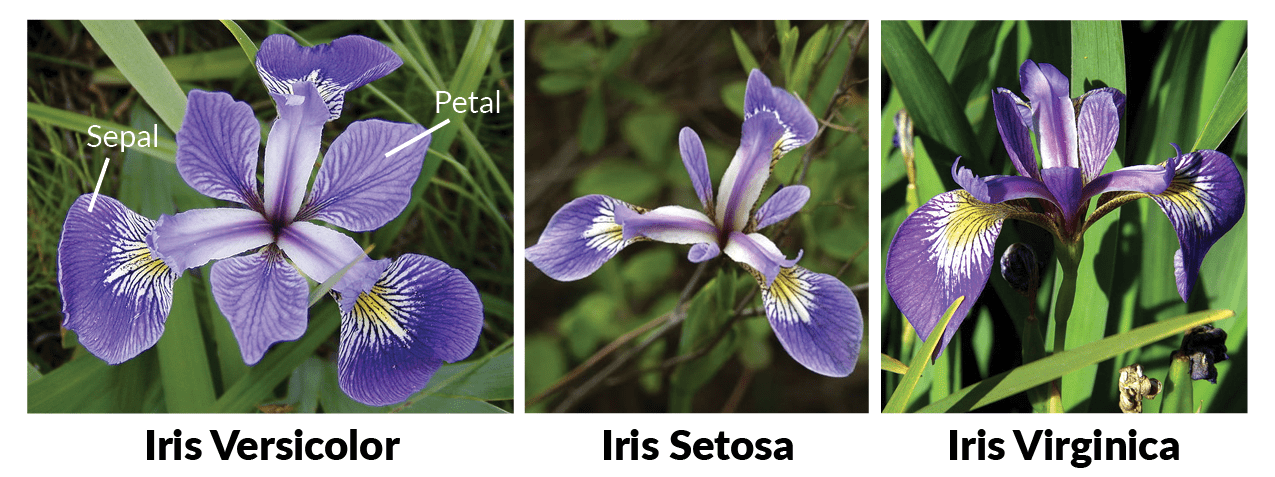
\includegraphics{figs/iris.png}
\caption{iris.png}
\end{figure}

    \begin{itemize}
\tightlist
\item
  Unlike last week, we will \textbf{NOT} work with the actual images,
  but rather with the numerical information extracted from samples.
\end{itemize}

    \begin{itemize}
\tightlist
\item
  First, we need to install \textbf{sklearn}:
\end{itemize}

    \begin{Verbatim}[commandchars=\\\{\}]
{\color{incolor}In [{\color{incolor}2}]:} \PY{o}{!}pip install sklearn
\end{Verbatim}


    \begin{Verbatim}[commandchars=\\\{\}]
Collecting sklearn
  Downloading https://files.pythonhosted.org/packages/1e/7a/dbb3be0ce9bd5c8b7e3d87328e79063f8b263b2b1bfa4774cb1147bfcd3f/sklearn-0.0.tar.gz
Requirement already satisfied: scikit-learn in c:\textbackslash{}anaconda\textbackslash{}lib\textbackslash{}site-packages (from sklearn) (0.20.3)
Requirement already satisfied: scipy>=0.13.3 in c:\textbackslash{}anaconda\textbackslash{}lib\textbackslash{}site-packages (from scikit-learn->sklearn) (1.2.1)
Requirement already satisfied: numpy>=1.8.2 in c:\textbackslash{}anaconda\textbackslash{}lib\textbackslash{}site-packages (from scikit-learn->sklearn) (1.16.2)
Building wheels for collected packages: sklearn
  Building wheel for sklearn (setup.py): started
  Building wheel for sklearn (setup.py): finished with status 'done'
  Stored in directory: C:\textbackslash{}Users\textbackslash{}CM8738\textbackslash{}AppData\textbackslash{}Local\textbackslash{}pip\textbackslash{}Cache\textbackslash{}wheels\textbackslash{}76\textbackslash{}03\textbackslash{}bb\textbackslash{}589d421d27431bcd2c6da284d5f2286c8e3b2ea3cf1594c074
Successfully built sklearn
Installing collected packages: sklearn
Successfully installed sklearn-0.0

    \end{Verbatim}

    \begin{itemize}
\tightlist
\item
  Then, we can load the iris dataset:
\end{itemize}

    \begin{Verbatim}[commandchars=\\\{\}]
{\color{incolor}In [{\color{incolor}3}]:} \PY{c+c1}{\PYZsh{}\PYZsh{} Load iris dataset}
        \PY{k+kn}{from} \PY{n+nn}{sklearn} \PY{k}{import} \PY{n}{datasets}
        \PY{n}{iris} \PY{o}{=} \PY{n}{datasets}\PY{o}{.}\PY{n}{load\PYZus{}iris}\PY{p}{(}\PY{p}{)}
        \PY{n+nb}{print}\PY{p}{(}\PY{n+nb}{type}\PY{p}{(}\PY{n}{iris}\PY{p}{)}\PY{p}{)}
\end{Verbatim}


    \begin{Verbatim}[commandchars=\\\{\}]
<class 'sklearn.utils.Bunch'>

    \end{Verbatim}

    \begin{itemize}
\tightlist
\item
  The dataset is contained on a \textbf{dictionary-like} structure
  referred to as \textbf{sklearn.utils.Bunch}.
\end{itemize}

    \begin{itemize}
\tightlist
\item
  If you print it, you will see a lot of things contained:
\end{itemize}

    \begin{Verbatim}[commandchars=\\\{\}]
{\color{incolor}In [{\color{incolor}4}]:} \PY{n+nb}{print}\PY{p}{(}\PY{n}{iris}\PY{p}{)}
\end{Verbatim}


    \begin{Verbatim}[commandchars=\\\{\}]
\{'data': array([[5.1, 3.5, 1.4, 0.2],
       [4.9, 3. , 1.4, 0.2],
       [4.7, 3.2, 1.3, 0.2],
       [4.6, 3.1, 1.5, 0.2],
       [5. , 3.6, 1.4, 0.2],
       [5.4, 3.9, 1.7, 0.4],
       [4.6, 3.4, 1.4, 0.3],
       [5. , 3.4, 1.5, 0.2],
       [4.4, 2.9, 1.4, 0.2],
       [4.9, 3.1, 1.5, 0.1],
       [5.4, 3.7, 1.5, 0.2],
       [4.8, 3.4, 1.6, 0.2],
       [4.8, 3. , 1.4, 0.1],
       [4.3, 3. , 1.1, 0.1],
       [5.8, 4. , 1.2, 0.2],
       [5.7, 4.4, 1.5, 0.4],
       [5.4, 3.9, 1.3, 0.4],
       [5.1, 3.5, 1.4, 0.3],
       [5.7, 3.8, 1.7, 0.3],
       [5.1, 3.8, 1.5, 0.3],
       [5.4, 3.4, 1.7, 0.2],
       [5.1, 3.7, 1.5, 0.4],
       [4.6, 3.6, 1. , 0.2],
       [5.1, 3.3, 1.7, 0.5],
       [4.8, 3.4, 1.9, 0.2],
       [5. , 3. , 1.6, 0.2],
       [5. , 3.4, 1.6, 0.4],
       [5.2, 3.5, 1.5, 0.2],
       [5.2, 3.4, 1.4, 0.2],
       [4.7, 3.2, 1.6, 0.2],
       [4.8, 3.1, 1.6, 0.2],
       [5.4, 3.4, 1.5, 0.4],
       [5.2, 4.1, 1.5, 0.1],
       [5.5, 4.2, 1.4, 0.2],
       [4.9, 3.1, 1.5, 0.2],
       [5. , 3.2, 1.2, 0.2],
       [5.5, 3.5, 1.3, 0.2],
       [4.9, 3.6, 1.4, 0.1],
       [4.4, 3. , 1.3, 0.2],
       [5.1, 3.4, 1.5, 0.2],
       [5. , 3.5, 1.3, 0.3],
       [4.5, 2.3, 1.3, 0.3],
       [4.4, 3.2, 1.3, 0.2],
       [5. , 3.5, 1.6, 0.6],
       [5.1, 3.8, 1.9, 0.4],
       [4.8, 3. , 1.4, 0.3],
       [5.1, 3.8, 1.6, 0.2],
       [4.6, 3.2, 1.4, 0.2],
       [5.3, 3.7, 1.5, 0.2],
       [5. , 3.3, 1.4, 0.2],
       [7. , 3.2, 4.7, 1.4],
       [6.4, 3.2, 4.5, 1.5],
       [6.9, 3.1, 4.9, 1.5],
       [5.5, 2.3, 4. , 1.3],
       [6.5, 2.8, 4.6, 1.5],
       [5.7, 2.8, 4.5, 1.3],
       [6.3, 3.3, 4.7, 1.6],
       [4.9, 2.4, 3.3, 1. ],
       [6.6, 2.9, 4.6, 1.3],
       [5.2, 2.7, 3.9, 1.4],
       [5. , 2. , 3.5, 1. ],
       [5.9, 3. , 4.2, 1.5],
       [6. , 2.2, 4. , 1. ],
       [6.1, 2.9, 4.7, 1.4],
       [5.6, 2.9, 3.6, 1.3],
       [6.7, 3.1, 4.4, 1.4],
       [5.6, 3. , 4.5, 1.5],
       [5.8, 2.7, 4.1, 1. ],
       [6.2, 2.2, 4.5, 1.5],
       [5.6, 2.5, 3.9, 1.1],
       [5.9, 3.2, 4.8, 1.8],
       [6.1, 2.8, 4. , 1.3],
       [6.3, 2.5, 4.9, 1.5],
       [6.1, 2.8, 4.7, 1.2],
       [6.4, 2.9, 4.3, 1.3],
       [6.6, 3. , 4.4, 1.4],
       [6.8, 2.8, 4.8, 1.4],
       [6.7, 3. , 5. , 1.7],
       [6. , 2.9, 4.5, 1.5],
       [5.7, 2.6, 3.5, 1. ],
       [5.5, 2.4, 3.8, 1.1],
       [5.5, 2.4, 3.7, 1. ],
       [5.8, 2.7, 3.9, 1.2],
       [6. , 2.7, 5.1, 1.6],
       [5.4, 3. , 4.5, 1.5],
       [6. , 3.4, 4.5, 1.6],
       [6.7, 3.1, 4.7, 1.5],
       [6.3, 2.3, 4.4, 1.3],
       [5.6, 3. , 4.1, 1.3],
       [5.5, 2.5, 4. , 1.3],
       [5.5, 2.6, 4.4, 1.2],
       [6.1, 3. , 4.6, 1.4],
       [5.8, 2.6, 4. , 1.2],
       [5. , 2.3, 3.3, 1. ],
       [5.6, 2.7, 4.2, 1.3],
       [5.7, 3. , 4.2, 1.2],
       [5.7, 2.9, 4.2, 1.3],
       [6.2, 2.9, 4.3, 1.3],
       [5.1, 2.5, 3. , 1.1],
       [5.7, 2.8, 4.1, 1.3],
       [6.3, 3.3, 6. , 2.5],
       [5.8, 2.7, 5.1, 1.9],
       [7.1, 3. , 5.9, 2.1],
       [6.3, 2.9, 5.6, 1.8],
       [6.5, 3. , 5.8, 2.2],
       [7.6, 3. , 6.6, 2.1],
       [4.9, 2.5, 4.5, 1.7],
       [7.3, 2.9, 6.3, 1.8],
       [6.7, 2.5, 5.8, 1.8],
       [7.2, 3.6, 6.1, 2.5],
       [6.5, 3.2, 5.1, 2. ],
       [6.4, 2.7, 5.3, 1.9],
       [6.8, 3. , 5.5, 2.1],
       [5.7, 2.5, 5. , 2. ],
       [5.8, 2.8, 5.1, 2.4],
       [6.4, 3.2, 5.3, 2.3],
       [6.5, 3. , 5.5, 1.8],
       [7.7, 3.8, 6.7, 2.2],
       [7.7, 2.6, 6.9, 2.3],
       [6. , 2.2, 5. , 1.5],
       [6.9, 3.2, 5.7, 2.3],
       [5.6, 2.8, 4.9, 2. ],
       [7.7, 2.8, 6.7, 2. ],
       [6.3, 2.7, 4.9, 1.8],
       [6.7, 3.3, 5.7, 2.1],
       [7.2, 3.2, 6. , 1.8],
       [6.2, 2.8, 4.8, 1.8],
       [6.1, 3. , 4.9, 1.8],
       [6.4, 2.8, 5.6, 2.1],
       [7.2, 3. , 5.8, 1.6],
       [7.4, 2.8, 6.1, 1.9],
       [7.9, 3.8, 6.4, 2. ],
       [6.4, 2.8, 5.6, 2.2],
       [6.3, 2.8, 5.1, 1.5],
       [6.1, 2.6, 5.6, 1.4],
       [7.7, 3. , 6.1, 2.3],
       [6.3, 3.4, 5.6, 2.4],
       [6.4, 3.1, 5.5, 1.8],
       [6. , 3. , 4.8, 1.8],
       [6.9, 3.1, 5.4, 2.1],
       [6.7, 3.1, 5.6, 2.4],
       [6.9, 3.1, 5.1, 2.3],
       [5.8, 2.7, 5.1, 1.9],
       [6.8, 3.2, 5.9, 2.3],
       [6.7, 3.3, 5.7, 2.5],
       [6.7, 3. , 5.2, 2.3],
       [6.3, 2.5, 5. , 1.9],
       [6.5, 3. , 5.2, 2. ],
       [6.2, 3.4, 5.4, 2.3],
       [5.9, 3. , 5.1, 1.8]]), 'target': array([0, 0, 0, 0, 0, 0, 0, 0, 0, 0, 0, 0, 0, 0, 0, 0, 0, 0, 0, 0, 0, 0,
       0, 0, 0, 0, 0, 0, 0, 0, 0, 0, 0, 0, 0, 0, 0, 0, 0, 0, 0, 0, 0, 0,
       0, 0, 0, 0, 0, 0, 1, 1, 1, 1, 1, 1, 1, 1, 1, 1, 1, 1, 1, 1, 1, 1,
       1, 1, 1, 1, 1, 1, 1, 1, 1, 1, 1, 1, 1, 1, 1, 1, 1, 1, 1, 1, 1, 1,
       1, 1, 1, 1, 1, 1, 1, 1, 1, 1, 1, 1, 2, 2, 2, 2, 2, 2, 2, 2, 2, 2,
       2, 2, 2, 2, 2, 2, 2, 2, 2, 2, 2, 2, 2, 2, 2, 2, 2, 2, 2, 2, 2, 2,
       2, 2, 2, 2, 2, 2, 2, 2, 2, 2, 2, 2, 2, 2, 2, 2, 2, 2]), 'target\_names': array(['setosa', 'versicolor', 'virginica'], dtype='<U10'), 'DESCR': '.. \_iris\_dataset:\textbackslash{}n\textbackslash{}nIris plants dataset\textbackslash{}n--------------------\textbackslash{}n\textbackslash{}n**Data Set Characteristics:**\textbackslash{}n\textbackslash{}n    :Number of Instances: 150 (50 in each of three classes)\textbackslash{}n    :Number of Attributes: 4 numeric, predictive attributes and the class\textbackslash{}n    :Attribute Information:\textbackslash{}n        - sepal length in cm\textbackslash{}n        - sepal width in cm\textbackslash{}n        - petal length in cm\textbackslash{}n        - petal width in cm\textbackslash{}n        - class:\textbackslash{}n                - Iris-Setosa\textbackslash{}n                - Iris-Versicolour\textbackslash{}n                - Iris-Virginica\textbackslash{}n                \textbackslash{}n    :Summary Statistics:\textbackslash{}n\textbackslash{}n    ============== ==== ==== ======= ===== ====================\textbackslash{}n                    Min  Max   Mean    SD   Class Correlation\textbackslash{}n    ============== ==== ==== ======= ===== ====================\textbackslash{}n    sepal length:   4.3  7.9   5.84   0.83    0.7826\textbackslash{}n    sepal width:    2.0  4.4   3.05   0.43   -0.4194\textbackslash{}n    petal length:   1.0  6.9   3.76   1.76    0.9490  (high!)\textbackslash{}n    petal width:    0.1  2.5   1.20   0.76    0.9565  (high!)\textbackslash{}n    ============== ==== ==== ======= ===== ====================\textbackslash{}n\textbackslash{}n    :Missing Attribute Values: None\textbackslash{}n    :Class Distribution: 33.3\% for each of 3 classes.\textbackslash{}n    :Creator: R.A. Fisher\textbackslash{}n    :Donor: Michael Marshall (MARSHALL\%PLU@io.arc.nasa.gov)\textbackslash{}n    :Date: July, 1988\textbackslash{}n\textbackslash{}nThe famous Iris database, first used by Sir R.A. Fisher. The dataset is taken\textbackslash{}nfrom Fisher\textbackslash{}'s paper. Note that it\textbackslash{}'s the same as in R, but not as in the UCI\textbackslash{}nMachine Learning Repository, which has two wrong data points.\textbackslash{}n\textbackslash{}nThis is perhaps the best known database to be found in the\textbackslash{}npattern recognition literature.  Fisher\textbackslash{}'s paper is a classic in the field and\textbackslash{}nis referenced frequently to this day.  (See Duda \& Hart, for example.)  The\textbackslash{}ndata set contains 3 classes of 50 instances each, where each class refers to a\textbackslash{}ntype of iris plant.  One class is linearly separable from the other 2; the\textbackslash{}nlatter are NOT linearly separable from each other.\textbackslash{}n\textbackslash{}n.. topic:: References\textbackslash{}n\textbackslash{}n   - Fisher, R.A. "The use of multiple measurements in taxonomic problems"\textbackslash{}n     Annual Eugenics, 7, Part II, 179-188 (1936); also in "Contributions to\textbackslash{}n     Mathematical Statistics" (John Wiley, NY, 1950).\textbackslash{}n   - Duda, R.O., \& Hart, P.E. (1973) Pattern Classification and Scene Analysis.\textbackslash{}n     (Q327.D83) John Wiley \& Sons.  ISBN 0-471-22361-1.  See page 218.\textbackslash{}n   - Dasarathy, B.V. (1980) "Nosing Around the Neighborhood: A New System\textbackslash{}n     Structure and Classification Rule for Recognition in Partially Exposed\textbackslash{}n     Environments".  IEEE Transactions on Pattern Analysis and Machine\textbackslash{}n     Intelligence, Vol. PAMI-2, No. 1, 67-71.\textbackslash{}n   - Gates, G.W. (1972) "The Reduced Nearest Neighbor Rule".  IEEE Transactions\textbackslash{}n     on Information Theory, May 1972, 431-433.\textbackslash{}n   - See also: 1988 MLC Proceedings, 54-64.  Cheeseman et al"s AUTOCLASS II\textbackslash{}n     conceptual clustering system finds 3 classes in the data.\textbackslash{}n   - Many, many more {\ldots}', 'feature\_names': ['sepal length (cm)', 'sepal width (cm)', 'petal length (cm)', 'petal width (cm)'], 'filename': 'C:\textbackslash{}\textbackslash{}Anaconda\textbackslash{}\textbackslash{}lib\textbackslash{}\textbackslash{}site-packages\textbackslash{}\textbackslash{}sklearn\textbackslash{}\textbackslash{}datasets\textbackslash{}\textbackslash{}data\textbackslash{}\textbackslash{}iris.csv'\}

    \end{Verbatim}

    \begin{itemize}
\tightlist
\item
  Therefore, we need to extract each index of this dictionary into a
  different variables to understand and analyse them separately.
\end{itemize}

    \begin{itemize}
\tightlist
\item
  First, we will import the data:
\end{itemize}

    \begin{Verbatim}[commandchars=\\\{\}]
{\color{incolor}In [{\color{incolor}5}]:} \PY{n}{data} \PY{o}{=} \PY{n}{iris}\PY{p}{[}\PY{l+s+s1}{\PYZsq{}}\PY{l+s+s1}{data}\PY{l+s+s1}{\PYZsq{}}\PY{p}{]}
        \PY{n+nb}{print}\PY{p}{(}\PY{n}{data}\PY{p}{,} \PY{n+nb}{type}\PY{p}{(}\PY{n}{data}\PY{p}{)}\PY{p}{,} \PY{n}{data}\PY{o}{.}\PY{n}{shape}\PY{p}{)}
\end{Verbatim}


    \begin{Verbatim}[commandchars=\\\{\}]
[[5.1 3.5 1.4 0.2]
 [4.9 3.  1.4 0.2]
 [4.7 3.2 1.3 0.2]
 [4.6 3.1 1.5 0.2]
 [5.  3.6 1.4 0.2]
 [5.4 3.9 1.7 0.4]
 [4.6 3.4 1.4 0.3]
 [5.  3.4 1.5 0.2]
 [4.4 2.9 1.4 0.2]
 [4.9 3.1 1.5 0.1]
 [5.4 3.7 1.5 0.2]
 [4.8 3.4 1.6 0.2]
 [4.8 3.  1.4 0.1]
 [4.3 3.  1.1 0.1]
 [5.8 4.  1.2 0.2]
 [5.7 4.4 1.5 0.4]
 [5.4 3.9 1.3 0.4]
 [5.1 3.5 1.4 0.3]
 [5.7 3.8 1.7 0.3]
 [5.1 3.8 1.5 0.3]
 [5.4 3.4 1.7 0.2]
 [5.1 3.7 1.5 0.4]
 [4.6 3.6 1.  0.2]
 [5.1 3.3 1.7 0.5]
 [4.8 3.4 1.9 0.2]
 [5.  3.  1.6 0.2]
 [5.  3.4 1.6 0.4]
 [5.2 3.5 1.5 0.2]
 [5.2 3.4 1.4 0.2]
 [4.7 3.2 1.6 0.2]
 [4.8 3.1 1.6 0.2]
 [5.4 3.4 1.5 0.4]
 [5.2 4.1 1.5 0.1]
 [5.5 4.2 1.4 0.2]
 [4.9 3.1 1.5 0.2]
 [5.  3.2 1.2 0.2]
 [5.5 3.5 1.3 0.2]
 [4.9 3.6 1.4 0.1]
 [4.4 3.  1.3 0.2]
 [5.1 3.4 1.5 0.2]
 [5.  3.5 1.3 0.3]
 [4.5 2.3 1.3 0.3]
 [4.4 3.2 1.3 0.2]
 [5.  3.5 1.6 0.6]
 [5.1 3.8 1.9 0.4]
 [4.8 3.  1.4 0.3]
 [5.1 3.8 1.6 0.2]
 [4.6 3.2 1.4 0.2]
 [5.3 3.7 1.5 0.2]
 [5.  3.3 1.4 0.2]
 [7.  3.2 4.7 1.4]
 [6.4 3.2 4.5 1.5]
 [6.9 3.1 4.9 1.5]
 [5.5 2.3 4.  1.3]
 [6.5 2.8 4.6 1.5]
 [5.7 2.8 4.5 1.3]
 [6.3 3.3 4.7 1.6]
 [4.9 2.4 3.3 1. ]
 [6.6 2.9 4.6 1.3]
 [5.2 2.7 3.9 1.4]
 [5.  2.  3.5 1. ]
 [5.9 3.  4.2 1.5]
 [6.  2.2 4.  1. ]
 [6.1 2.9 4.7 1.4]
 [5.6 2.9 3.6 1.3]
 [6.7 3.1 4.4 1.4]
 [5.6 3.  4.5 1.5]
 [5.8 2.7 4.1 1. ]
 [6.2 2.2 4.5 1.5]
 [5.6 2.5 3.9 1.1]
 [5.9 3.2 4.8 1.8]
 [6.1 2.8 4.  1.3]
 [6.3 2.5 4.9 1.5]
 [6.1 2.8 4.7 1.2]
 [6.4 2.9 4.3 1.3]
 [6.6 3.  4.4 1.4]
 [6.8 2.8 4.8 1.4]
 [6.7 3.  5.  1.7]
 [6.  2.9 4.5 1.5]
 [5.7 2.6 3.5 1. ]
 [5.5 2.4 3.8 1.1]
 [5.5 2.4 3.7 1. ]
 [5.8 2.7 3.9 1.2]
 [6.  2.7 5.1 1.6]
 [5.4 3.  4.5 1.5]
 [6.  3.4 4.5 1.6]
 [6.7 3.1 4.7 1.5]
 [6.3 2.3 4.4 1.3]
 [5.6 3.  4.1 1.3]
 [5.5 2.5 4.  1.3]
 [5.5 2.6 4.4 1.2]
 [6.1 3.  4.6 1.4]
 [5.8 2.6 4.  1.2]
 [5.  2.3 3.3 1. ]
 [5.6 2.7 4.2 1.3]
 [5.7 3.  4.2 1.2]
 [5.7 2.9 4.2 1.3]
 [6.2 2.9 4.3 1.3]
 [5.1 2.5 3.  1.1]
 [5.7 2.8 4.1 1.3]
 [6.3 3.3 6.  2.5]
 [5.8 2.7 5.1 1.9]
 [7.1 3.  5.9 2.1]
 [6.3 2.9 5.6 1.8]
 [6.5 3.  5.8 2.2]
 [7.6 3.  6.6 2.1]
 [4.9 2.5 4.5 1.7]
 [7.3 2.9 6.3 1.8]
 [6.7 2.5 5.8 1.8]
 [7.2 3.6 6.1 2.5]
 [6.5 3.2 5.1 2. ]
 [6.4 2.7 5.3 1.9]
 [6.8 3.  5.5 2.1]
 [5.7 2.5 5.  2. ]
 [5.8 2.8 5.1 2.4]
 [6.4 3.2 5.3 2.3]
 [6.5 3.  5.5 1.8]
 [7.7 3.8 6.7 2.2]
 [7.7 2.6 6.9 2.3]
 [6.  2.2 5.  1.5]
 [6.9 3.2 5.7 2.3]
 [5.6 2.8 4.9 2. ]
 [7.7 2.8 6.7 2. ]
 [6.3 2.7 4.9 1.8]
 [6.7 3.3 5.7 2.1]
 [7.2 3.2 6.  1.8]
 [6.2 2.8 4.8 1.8]
 [6.1 3.  4.9 1.8]
 [6.4 2.8 5.6 2.1]
 [7.2 3.  5.8 1.6]
 [7.4 2.8 6.1 1.9]
 [7.9 3.8 6.4 2. ]
 [6.4 2.8 5.6 2.2]
 [6.3 2.8 5.1 1.5]
 [6.1 2.6 5.6 1.4]
 [7.7 3.  6.1 2.3]
 [6.3 3.4 5.6 2.4]
 [6.4 3.1 5.5 1.8]
 [6.  3.  4.8 1.8]
 [6.9 3.1 5.4 2.1]
 [6.7 3.1 5.6 2.4]
 [6.9 3.1 5.1 2.3]
 [5.8 2.7 5.1 1.9]
 [6.8 3.2 5.9 2.3]
 [6.7 3.3 5.7 2.5]
 [6.7 3.  5.2 2.3]
 [6.3 2.5 5.  1.9]
 [6.5 3.  5.2 2. ]
 [6.2 3.4 5.4 2.3]
 [5.9 3.  5.1 1.8]] <class 'numpy.ndarray'> (150, 4)

    \end{Verbatim}

    \begin{Verbatim}[commandchars=\\\{\}]
{\color{incolor}In [{\color{incolor}7}]:} \PY{n+nb}{set}\PY{p}{(}\PY{n}{iris}\PY{p}{)}
\end{Verbatim}


\begin{Verbatim}[commandchars=\\\{\}]
{\color{outcolor}Out[{\color{outcolor}7}]:} \{'DESCR', 'data', 'feature\_names', 'filename', 'target', 'target\_names'\}
\end{Verbatim}
            
    \begin{itemize}
\tightlist
\item
  The data is stored in a \emph{numpy array} of 150 rows and 4 columns,
  each corresponding to the measurements of a flower.
\end{itemize}

    \begin{itemize}
\tightlist
\item
  Then, we will import the headers of the data:
\end{itemize}

    \begin{Verbatim}[commandchars=\\\{\}]
{\color{incolor}In [{\color{incolor}6}]:} \PY{n}{header} \PY{o}{=} \PY{n}{iris}\PY{p}{[}\PY{l+s+s1}{\PYZsq{}}\PY{l+s+s1}{feature\PYZus{}names}\PY{l+s+s1}{\PYZsq{}}\PY{p}{]}
        \PY{n+nb}{print}\PY{p}{(}\PY{n}{header}\PY{p}{,} \PY{n+nb}{type}\PY{p}{(}\PY{n}{header}\PY{p}{)}\PY{p}{)}
\end{Verbatim}


    \begin{Verbatim}[commandchars=\\\{\}]
['sepal length (cm)', 'sepal width (cm)', 'petal length (cm)', 'petal width (cm)'] <class 'list'>

    \end{Verbatim}

    \begin{itemize}
\tightlist
\item
  \textbf{Why do you think the data and the header are stored
  separately?}
\end{itemize}

    \begin{itemize}
\tightlist
\item
  Afterwards, we will import the \textbf{class/target}:
\end{itemize}

    \begin{Verbatim}[commandchars=\\\{\}]
{\color{incolor}In [{\color{incolor}8}]:} \PY{n}{target} \PY{o}{=} \PY{n}{iris}\PY{p}{[}\PY{l+s+s1}{\PYZsq{}}\PY{l+s+s1}{target}\PY{l+s+s1}{\PYZsq{}}\PY{p}{]}
        \PY{n+nb}{print}\PY{p}{(}\PY{n}{target}\PY{p}{,} \PY{n+nb}{type}\PY{p}{(}\PY{n}{target}\PY{p}{)}\PY{p}{,} \PY{n}{target}\PY{o}{.}\PY{n}{shape}\PY{p}{)}
\end{Verbatim}


    \begin{Verbatim}[commandchars=\\\{\}]
[0 0 0 0 0 0 0 0 0 0 0 0 0 0 0 0 0 0 0 0 0 0 0 0 0 0 0 0 0 0 0 0 0 0 0 0 0
 0 0 0 0 0 0 0 0 0 0 0 0 0 1 1 1 1 1 1 1 1 1 1 1 1 1 1 1 1 1 1 1 1 1 1 1 1
 1 1 1 1 1 1 1 1 1 1 1 1 1 1 1 1 1 1 1 1 1 1 1 1 1 1 2 2 2 2 2 2 2 2 2 2 2
 2 2 2 2 2 2 2 2 2 2 2 2 2 2 2 2 2 2 2 2 2 2 2 2 2 2 2 2 2 2 2 2 2 2 2 2 2
 2 2] <class 'numpy.ndarray'> (150,)

    \end{Verbatim}

    \begin{itemize}
\tightlist
\item
  The class/target is a \emph{numpy array} which contains the
  \textbf{category} of each flowers.
\end{itemize}

    \begin{itemize}
\tightlist
\item
  Each sample is labelled as \(0\), \(1\) or \(2\) instead of the iris
  type since the labels can be better used as numbers.
\end{itemize}

    \begin{itemize}
\tightlist
\item
  A separate key called \textbf{target\_names} contains the name
  corresponding to each numerical label.
\end{itemize}

    \begin{Verbatim}[commandchars=\\\{\}]
{\color{incolor}In [{\color{incolor}9}]:} \PY{n}{target\PYZus{}names} \PY{o}{=} \PY{n}{iris}\PY{p}{[}\PY{l+s+s1}{\PYZsq{}}\PY{l+s+s1}{target\PYZus{}names}\PY{l+s+s1}{\PYZsq{}}\PY{p}{]}
        \PY{n+nb}{print}\PY{p}{(}\PY{n}{target\PYZus{}names}\PY{p}{,} \PY{n+nb}{type}\PY{p}{(}\PY{n}{target\PYZus{}names}\PY{p}{)}\PY{p}{,} \PY{n}{target\PYZus{}names}\PY{o}{.}\PY{n}{shape}\PY{p}{)}
\end{Verbatim}


    \begin{Verbatim}[commandchars=\\\{\}]
['setosa' 'versicolor' 'virginica'] <class 'numpy.ndarray'> (3,)

    \end{Verbatim}

    \begin{itemize}
\tightlist
\item
  Finally, just in case you are interested, there is an entry containing
  the description of the dataset (a string):
\end{itemize}

    \begin{Verbatim}[commandchars=\\\{\}]
{\color{incolor}In [{\color{incolor}10}]:} \PY{n}{iris}\PY{p}{[}\PY{l+s+s1}{\PYZsq{}}\PY{l+s+s1}{DESCR}\PY{l+s+s1}{\PYZsq{}}\PY{p}{]}
\end{Verbatim}


\begin{Verbatim}[commandchars=\\\{\}]
{\color{outcolor}Out[{\color{outcolor}10}]:} '.. \_iris\_dataset:\textbackslash{}n\textbackslash{}nIris plants dataset\textbackslash{}n--------------------\textbackslash{}n\textbackslash{}n**Data Set Characteristics:**\textbackslash{}n\textbackslash{}n    :Number of Instances: 150 (50 in each of three classes)\textbackslash{}n    :Number of Attributes: 4 numeric, predictive attributes and the class\textbackslash{}n    :Attribute Information:\textbackslash{}n        - sepal length in cm\textbackslash{}n        - sepal width in cm\textbackslash{}n        - petal length in cm\textbackslash{}n        - petal width in cm\textbackslash{}n        - class:\textbackslash{}n                - Iris-Setosa\textbackslash{}n                - Iris-Versicolour\textbackslash{}n                - Iris-Virginica\textbackslash{}n                \textbackslash{}n    :Summary Statistics:\textbackslash{}n\textbackslash{}n    ============== ==== ==== ======= ===== ====================\textbackslash{}n                    Min  Max   Mean    SD   Class Correlation\textbackslash{}n    ============== ==== ==== ======= ===== ====================\textbackslash{}n    sepal length:   4.3  7.9   5.84   0.83    0.7826\textbackslash{}n    sepal width:    2.0  4.4   3.05   0.43   -0.4194\textbackslash{}n    petal length:   1.0  6.9   3.76   1.76    0.9490  (high!)\textbackslash{}n    petal width:    0.1  2.5   1.20   0.76    0.9565  (high!)\textbackslash{}n    ============== ==== ==== ======= ===== ====================\textbackslash{}n\textbackslash{}n    :Missing Attribute Values: None\textbackslash{}n    :Class Distribution: 33.3\% for each of 3 classes.\textbackslash{}n    :Creator: R.A. Fisher\textbackslash{}n    :Donor: Michael Marshall (MARSHALL\%PLU@io.arc.nasa.gov)\textbackslash{}n    :Date: July, 1988\textbackslash{}n\textbackslash{}nThe famous Iris database, first used by Sir R.A. Fisher. The dataset is taken\textbackslash{}nfrom Fisher\textbackslash{}'s paper. Note that it\textbackslash{}'s the same as in R, but not as in the UCI\textbackslash{}nMachine Learning Repository, which has two wrong data points.\textbackslash{}n\textbackslash{}nThis is perhaps the best known database to be found in the\textbackslash{}npattern recognition literature.  Fisher\textbackslash{}'s paper is a classic in the field and\textbackslash{}nis referenced frequently to this day.  (See Duda \& Hart, for example.)  The\textbackslash{}ndata set contains 3 classes of 50 instances each, where each class refers to a\textbackslash{}ntype of iris plant.  One class is linearly separable from the other 2; the\textbackslash{}nlatter are NOT linearly separable from each other.\textbackslash{}n\textbackslash{}n.. topic:: References\textbackslash{}n\textbackslash{}n   - Fisher, R.A. "The use of multiple measurements in taxonomic problems"\textbackslash{}n     Annual Eugenics, 7, Part II, 179-188 (1936); also in "Contributions to\textbackslash{}n     Mathematical Statistics" (John Wiley, NY, 1950).\textbackslash{}n   - Duda, R.O., \& Hart, P.E. (1973) Pattern Classification and Scene Analysis.\textbackslash{}n     (Q327.D83) John Wiley \& Sons.  ISBN 0-471-22361-1.  See page 218.\textbackslash{}n   - Dasarathy, B.V. (1980) "Nosing Around the Neighborhood: A New System\textbackslash{}n     Structure and Classification Rule for Recognition in Partially Exposed\textbackslash{}n     Environments".  IEEE Transactions on Pattern Analysis and Machine\textbackslash{}n     Intelligence, Vol. PAMI-2, No. 1, 67-71.\textbackslash{}n   - Gates, G.W. (1972) "The Reduced Nearest Neighbor Rule".  IEEE Transactions\textbackslash{}n     on Information Theory, May 1972, 431-433.\textbackslash{}n   - See also: 1988 MLC Proceedings, 54-64.  Cheeseman et al"s AUTOCLASS II\textbackslash{}n     conceptual clustering system finds 3 classes in the data.\textbackslash{}n   - Many, many more {\ldots}'
\end{Verbatim}
            
    \hypertarget{wrangling-data}{%
\subsubsection{Wrangling Data}\label{wrangling-data}}

    \begin{itemize}
\tightlist
\item
  Accessing an individual entry of the dataset (along with its
  class/target):
\end{itemize}

    \begin{Verbatim}[commandchars=\\\{\}]
{\color{incolor}In [{\color{incolor}16}]:} \PY{n}{n} \PY{o}{=} \PY{l+m+mi}{89}
         \PY{n+nb}{print}\PY{p}{(}\PY{n}{data}\PY{p}{[}\PY{n}{n}\PY{p}{]}\PY{p}{,} \PY{n}{target}\PY{p}{[}\PY{n}{n}\PY{p}{]}\PY{p}{)}
\end{Verbatim}


    \begin{Verbatim}[commandchars=\\\{\}]
[5.5 2.5 4.  1.3] 1

    \end{Verbatim}

    \begin{itemize}
\tightlist
\item
  Creating a table for each iris type (``manually'')
\end{itemize}

    \begin{Verbatim}[commandchars=\\\{\}]
{\color{incolor}In [{\color{incolor}19}]:} \PY{n}{setosa} \PY{o}{=} \PY{n}{data}\PY{p}{[}\PY{l+m+mi}{0}\PY{p}{:}\PY{l+m+mi}{50}\PY{p}{]}
         \PY{n+nb}{print}\PY{p}{(}\PY{n}{setosa}\PY{p}{,} \PY{n}{setosa}\PY{o}{.}\PY{n}{shape}\PY{p}{)}
\end{Verbatim}


    \begin{Verbatim}[commandchars=\\\{\}]
[[5.1 3.5 1.4 0.2]
 [4.9 3.  1.4 0.2]
 [4.7 3.2 1.3 0.2]
 [4.6 3.1 1.5 0.2]
 [5.  3.6 1.4 0.2]
 [5.4 3.9 1.7 0.4]
 [4.6 3.4 1.4 0.3]
 [5.  3.4 1.5 0.2]
 [4.4 2.9 1.4 0.2]
 [4.9 3.1 1.5 0.1]
 [5.4 3.7 1.5 0.2]
 [4.8 3.4 1.6 0.2]
 [4.8 3.  1.4 0.1]
 [4.3 3.  1.1 0.1]
 [5.8 4.  1.2 0.2]
 [5.7 4.4 1.5 0.4]
 [5.4 3.9 1.3 0.4]
 [5.1 3.5 1.4 0.3]
 [5.7 3.8 1.7 0.3]
 [5.1 3.8 1.5 0.3]
 [5.4 3.4 1.7 0.2]
 [5.1 3.7 1.5 0.4]
 [4.6 3.6 1.  0.2]
 [5.1 3.3 1.7 0.5]
 [4.8 3.4 1.9 0.2]
 [5.  3.  1.6 0.2]
 [5.  3.4 1.6 0.4]
 [5.2 3.5 1.5 0.2]
 [5.2 3.4 1.4 0.2]
 [4.7 3.2 1.6 0.2]
 [4.8 3.1 1.6 0.2]
 [5.4 3.4 1.5 0.4]
 [5.2 4.1 1.5 0.1]
 [5.5 4.2 1.4 0.2]
 [4.9 3.1 1.5 0.2]
 [5.  3.2 1.2 0.2]
 [5.5 3.5 1.3 0.2]
 [4.9 3.6 1.4 0.1]
 [4.4 3.  1.3 0.2]
 [5.1 3.4 1.5 0.2]
 [5.  3.5 1.3 0.3]
 [4.5 2.3 1.3 0.3]
 [4.4 3.2 1.3 0.2]
 [5.  3.5 1.6 0.6]
 [5.1 3.8 1.9 0.4]
 [4.8 3.  1.4 0.3]
 [5.1 3.8 1.6 0.2]
 [4.6 3.2 1.4 0.2]
 [5.3 3.7 1.5 0.2]
 [5.  3.3 1.4 0.2]] (50, 4)

    \end{Verbatim}

    \begin{Verbatim}[commandchars=\\\{\}]
{\color{incolor}In [{\color{incolor}21}]:} \PY{c+c1}{\PYZsh{}\PYZsh{} Use this cell to create and print versicolor }
         \PY{c+c1}{\PYZsh{}\PYZsh{}  and virginica (with the shape)}
         \PY{n}{versicolor} \PY{o}{=} \PY{n}{data}\PY{p}{[}\PY{l+m+mi}{50}\PY{p}{:}\PY{l+m+mi}{100}\PY{p}{]}
         \PY{n}{virginica} \PY{o}{=} \PY{n}{data}\PY{p}{[}\PY{l+m+mi}{100}\PY{p}{:}\PY{l+m+mi}{150}\PY{p}{]}
         \PY{n+nb}{print}\PY{p}{(}\PY{n}{versicolor}\PY{p}{,}\PY{n}{versicolor}\PY{o}{.}\PY{n}{shape}\PY{p}{)}
         \PY{n+nb}{print}\PY{p}{(}\PY{n}{virginica}\PY{p}{,}\PY{n}{virginica}\PY{o}{.}\PY{n}{shape}\PY{p}{)}
\end{Verbatim}


    \begin{Verbatim}[commandchars=\\\{\}]
[[7.  3.2 4.7 1.4]
 [6.4 3.2 4.5 1.5]
 [6.9 3.1 4.9 1.5]
 [5.5 2.3 4.  1.3]
 [6.5 2.8 4.6 1.5]
 [5.7 2.8 4.5 1.3]
 [6.3 3.3 4.7 1.6]
 [4.9 2.4 3.3 1. ]
 [6.6 2.9 4.6 1.3]
 [5.2 2.7 3.9 1.4]
 [5.  2.  3.5 1. ]
 [5.9 3.  4.2 1.5]
 [6.  2.2 4.  1. ]
 [6.1 2.9 4.7 1.4]
 [5.6 2.9 3.6 1.3]
 [6.7 3.1 4.4 1.4]
 [5.6 3.  4.5 1.5]
 [5.8 2.7 4.1 1. ]
 [6.2 2.2 4.5 1.5]
 [5.6 2.5 3.9 1.1]
 [5.9 3.2 4.8 1.8]
 [6.1 2.8 4.  1.3]
 [6.3 2.5 4.9 1.5]
 [6.1 2.8 4.7 1.2]
 [6.4 2.9 4.3 1.3]
 [6.6 3.  4.4 1.4]
 [6.8 2.8 4.8 1.4]
 [6.7 3.  5.  1.7]
 [6.  2.9 4.5 1.5]
 [5.7 2.6 3.5 1. ]
 [5.5 2.4 3.8 1.1]
 [5.5 2.4 3.7 1. ]
 [5.8 2.7 3.9 1.2]
 [6.  2.7 5.1 1.6]
 [5.4 3.  4.5 1.5]
 [6.  3.4 4.5 1.6]
 [6.7 3.1 4.7 1.5]
 [6.3 2.3 4.4 1.3]
 [5.6 3.  4.1 1.3]
 [5.5 2.5 4.  1.3]
 [5.5 2.6 4.4 1.2]
 [6.1 3.  4.6 1.4]
 [5.8 2.6 4.  1.2]
 [5.  2.3 3.3 1. ]
 [5.6 2.7 4.2 1.3]
 [5.7 3.  4.2 1.2]
 [5.7 2.9 4.2 1.3]
 [6.2 2.9 4.3 1.3]
 [5.1 2.5 3.  1.1]
 [5.7 2.8 4.1 1.3]] (50, 4)
[[6.3 3.3 6.  2.5]
 [5.8 2.7 5.1 1.9]
 [7.1 3.  5.9 2.1]
 [6.3 2.9 5.6 1.8]
 [6.5 3.  5.8 2.2]
 [7.6 3.  6.6 2.1]
 [4.9 2.5 4.5 1.7]
 [7.3 2.9 6.3 1.8]
 [6.7 2.5 5.8 1.8]
 [7.2 3.6 6.1 2.5]
 [6.5 3.2 5.1 2. ]
 [6.4 2.7 5.3 1.9]
 [6.8 3.  5.5 2.1]
 [5.7 2.5 5.  2. ]
 [5.8 2.8 5.1 2.4]
 [6.4 3.2 5.3 2.3]
 [6.5 3.  5.5 1.8]
 [7.7 3.8 6.7 2.2]
 [7.7 2.6 6.9 2.3]
 [6.  2.2 5.  1.5]
 [6.9 3.2 5.7 2.3]
 [5.6 2.8 4.9 2. ]
 [7.7 2.8 6.7 2. ]
 [6.3 2.7 4.9 1.8]
 [6.7 3.3 5.7 2.1]
 [7.2 3.2 6.  1.8]
 [6.2 2.8 4.8 1.8]
 [6.1 3.  4.9 1.8]
 [6.4 2.8 5.6 2.1]
 [7.2 3.  5.8 1.6]
 [7.4 2.8 6.1 1.9]
 [7.9 3.8 6.4 2. ]
 [6.4 2.8 5.6 2.2]
 [6.3 2.8 5.1 1.5]
 [6.1 2.6 5.6 1.4]
 [7.7 3.  6.1 2.3]
 [6.3 3.4 5.6 2.4]
 [6.4 3.1 5.5 1.8]
 [6.  3.  4.8 1.8]
 [6.9 3.1 5.4 2.1]
 [6.7 3.1 5.6 2.4]
 [6.9 3.1 5.1 2.3]
 [5.8 2.7 5.1 1.9]
 [6.8 3.2 5.9 2.3]
 [6.7 3.3 5.7 2.5]
 [6.7 3.  5.2 2.3]
 [6.3 2.5 5.  1.9]
 [6.5 3.  5.2 2. ]
 [6.2 3.4 5.4 2.3]
 [5.9 3.  5.1 1.8]] (50, 4)

    \end{Verbatim}

    \begin{itemize}
\tightlist
\item
  Creating a table for each iris type (``automatically'')
\end{itemize}

    \begin{Verbatim}[commandchars=\\\{\}]
{\color{incolor}In [{\color{incolor}24}]:} \PY{c+c1}{\PYZsh{}\PYZsh{} In case that data is not in order or you don\PYZsq{}t want to count,}
         \PY{c+c1}{\PYZsh{}\PYZsh{} we can use this alternative:}
         \PY{k+kn}{import} \PY{n+nn}{numpy} \PY{k}{as} \PY{n+nn}{np}
         \PY{n}{setosa2} \PY{o}{=} \PY{n}{data}\PY{p}{[}\PY{n}{np}\PY{o}{.}\PY{n}{where}\PY{p}{(}\PY{n}{target}\PY{o}{==}\PY{l+m+mi}{0}\PY{p}{)}\PY{p}{]}
         \PY{n+nb}{print}\PY{p}{(}\PY{n}{setosa}\PY{p}{,} \PY{n}{setosa}\PY{o}{.}\PY{n}{shape}\PY{p}{)}
\end{Verbatim}


    \begin{Verbatim}[commandchars=\\\{\}]
[[5.1 3.5 1.4 0.2]
 [4.9 3.  1.4 0.2]
 [4.7 3.2 1.3 0.2]
 [4.6 3.1 1.5 0.2]
 [5.  3.6 1.4 0.2]
 [5.4 3.9 1.7 0.4]
 [4.6 3.4 1.4 0.3]
 [5.  3.4 1.5 0.2]
 [4.4 2.9 1.4 0.2]
 [4.9 3.1 1.5 0.1]
 [5.4 3.7 1.5 0.2]
 [4.8 3.4 1.6 0.2]
 [4.8 3.  1.4 0.1]
 [4.3 3.  1.1 0.1]
 [5.8 4.  1.2 0.2]
 [5.7 4.4 1.5 0.4]
 [5.4 3.9 1.3 0.4]
 [5.1 3.5 1.4 0.3]
 [5.7 3.8 1.7 0.3]
 [5.1 3.8 1.5 0.3]
 [5.4 3.4 1.7 0.2]
 [5.1 3.7 1.5 0.4]
 [4.6 3.6 1.  0.2]
 [5.1 3.3 1.7 0.5]
 [4.8 3.4 1.9 0.2]
 [5.  3.  1.6 0.2]
 [5.  3.4 1.6 0.4]
 [5.2 3.5 1.5 0.2]
 [5.2 3.4 1.4 0.2]
 [4.7 3.2 1.6 0.2]
 [4.8 3.1 1.6 0.2]
 [5.4 3.4 1.5 0.4]
 [5.2 4.1 1.5 0.1]
 [5.5 4.2 1.4 0.2]
 [4.9 3.1 1.5 0.2]
 [5.  3.2 1.2 0.2]
 [5.5 3.5 1.3 0.2]
 [4.9 3.6 1.4 0.1]
 [4.4 3.  1.3 0.2]
 [5.1 3.4 1.5 0.2]
 [5.  3.5 1.3 0.3]
 [4.5 2.3 1.3 0.3]
 [4.4 3.2 1.3 0.2]
 [5.  3.5 1.6 0.6]
 [5.1 3.8 1.9 0.4]
 [4.8 3.  1.4 0.3]
 [5.1 3.8 1.6 0.2]
 [4.6 3.2 1.4 0.2]
 [5.3 3.7 1.5 0.2]
 [5.  3.3 1.4 0.2]] (50, 4)

    \end{Verbatim}

    \begin{Verbatim}[commandchars=\\\{\}]
{\color{incolor}In [{\color{incolor}25}]:} \PY{c+c1}{\PYZsh{}\PYZsh{} Verify that we get the same}
         \PY{n}{setosa} \PY{o}{==} \PY{n}{setosa2}
\end{Verbatim}


\begin{Verbatim}[commandchars=\\\{\}]
{\color{outcolor}Out[{\color{outcolor}25}]:} array([[ True,  True,  True,  True],
                [ True,  True,  True,  True],
                [ True,  True,  True,  True],
                [ True,  True,  True,  True],
                [ True,  True,  True,  True],
                [ True,  True,  True,  True],
                [ True,  True,  True,  True],
                [ True,  True,  True,  True],
                [ True,  True,  True,  True],
                [ True,  True,  True,  True],
                [ True,  True,  True,  True],
                [ True,  True,  True,  True],
                [ True,  True,  True,  True],
                [ True,  True,  True,  True],
                [ True,  True,  True,  True],
                [ True,  True,  True,  True],
                [ True,  True,  True,  True],
                [ True,  True,  True,  True],
                [ True,  True,  True,  True],
                [ True,  True,  True,  True],
                [ True,  True,  True,  True],
                [ True,  True,  True,  True],
                [ True,  True,  True,  True],
                [ True,  True,  True,  True],
                [ True,  True,  True,  True],
                [ True,  True,  True,  True],
                [ True,  True,  True,  True],
                [ True,  True,  True,  True],
                [ True,  True,  True,  True],
                [ True,  True,  True,  True],
                [ True,  True,  True,  True],
                [ True,  True,  True,  True],
                [ True,  True,  True,  True],
                [ True,  True,  True,  True],
                [ True,  True,  True,  True],
                [ True,  True,  True,  True],
                [ True,  True,  True,  True],
                [ True,  True,  True,  True],
                [ True,  True,  True,  True],
                [ True,  True,  True,  True],
                [ True,  True,  True,  True],
                [ True,  True,  True,  True],
                [ True,  True,  True,  True],
                [ True,  True,  True,  True],
                [ True,  True,  True,  True],
                [ True,  True,  True,  True],
                [ True,  True,  True,  True],
                [ True,  True,  True,  True],
                [ True,  True,  True,  True],
                [ True,  True,  True,  True]])
\end{Verbatim}
            
    \begin{itemize}
\tightlist
\item
  Creating a new table with ``less'' columns (by column number):
\end{itemize}

    \begin{Verbatim}[commandchars=\\\{\}]
{\color{incolor}In [{\color{incolor}45}]:} \PY{c+c1}{\PYZsh{}\PYZsh{} creating a \PYZdq{}reduced\PYZdq{} table}
         \PY{c+c1}{\PYZsh{}\PYZsh{} with ony the first two columns}
         \PY{n+nb}{print}\PY{p}{(}\PY{n}{data}\PY{p}{[}\PY{l+m+mi}{0}\PY{p}{]}\PY{p}{)}
         \PY{n}{data\PYZus{}red1} \PY{o}{=} \PY{n}{data}\PY{p}{[}\PY{l+m+mi}{0}\PY{p}{,}\PY{o}{\PYZhy{}}\PY{l+m+mi}{3}\PY{p}{:}\PY{p}{]}
         \PY{n+nb}{print}\PY{p}{(}\PY{n}{data\PYZus{}red1}\PY{p}{,}\PY{n}{data\PYZus{}red1}\PY{o}{.}\PY{n}{shape}\PY{p}{)}
\end{Verbatim}


    \begin{Verbatim}[commandchars=\\\{\}]
[5.1 3.5 1.4 0.2]
[3.5 1.4 0.2] (3,)

    \end{Verbatim}

    \begin{Verbatim}[commandchars=\\\{\}]
{\color{incolor}In [{\color{incolor} }]:} \PY{c+c1}{\PYZsh{}\PYZsh{} Use this cell to create a new dataset called data\PYZus{}red2 }
        \PY{c+c1}{\PYZsh{}\PYZsh{} with the last two columns}
\end{Verbatim}


    \begin{Verbatim}[commandchars=\\\{\}]
{\color{incolor}In [{\color{incolor}60}]:} \PY{c+c1}{\PYZsh{}\PYZsh{} Use this cell to create a new dataset called data\PYZus{}red3 }
         \PY{c+c1}{\PYZsh{}\PYZsh{} with the first and the third columns}
         \PY{n}{data}\PY{p}{[}\PY{p}{:}\PY{p}{,}\PY{p}{[}\PY{l+m+mi}{0}\PY{p}{,}\PY{l+m+mi}{2}\PY{p}{]}\PY{p}{]}\PY{p}{[}\PY{p}{[}\PY{l+m+mi}{6}\PY{p}{,}\PY{l+m+mi}{7}\PY{p}{,}\PY{l+m+mi}{8}\PY{p}{]}\PY{p}{,}\PY{p}{:}\PY{p}{]}
\end{Verbatim}


\begin{Verbatim}[commandchars=\\\{\}]
{\color{outcolor}Out[{\color{outcolor}60}]:} array([[4.6, 1.4],
                [5. , 1.5],
                [4.4, 1.4]])
\end{Verbatim}
            
    \begin{Verbatim}[commandchars=\\\{\}]
{\color{incolor}In [{\color{incolor}61}]:} \PY{c+c1}{\PYZsh{}\PYZsh{} creating a \PYZdq{}reduced\PYZdq{} table with ony the first column}
         \PY{n}{col\PYZus{}0} \PY{o}{=} \PY{n}{data}\PY{p}{[}\PY{p}{:}\PY{p}{,}\PY{l+m+mi}{0}\PY{p}{]}
         \PY{n+nb}{print}\PY{p}{(}\PY{n}{col\PYZus{}0}\PY{p}{,}\PY{n}{col\PYZus{}0}\PY{o}{.}\PY{n}{shape}\PY{p}{)}
\end{Verbatim}


    \begin{Verbatim}[commandchars=\\\{\}]
[5.1 4.9 4.7 4.6 5.  5.4 4.6 5.  4.4 4.9 5.4 4.8 4.8 4.3 5.8 5.7 5.4 5.1
 5.7 5.1 5.4 5.1 4.6 5.1 4.8 5.  5.  5.2 5.2 4.7 4.8 5.4 5.2 5.5 4.9 5.
 5.5 4.9 4.4 5.1 5.  4.5 4.4 5.  5.1 4.8 5.1 4.6 5.3 5.  7.  6.4 6.9 5.5
 6.5 5.7 6.3 4.9 6.6 5.2 5.  5.9 6.  6.1 5.6 6.7 5.6 5.8 6.2 5.6 5.9 6.1
 6.3 6.1 6.4 6.6 6.8 6.7 6.  5.7 5.5 5.5 5.8 6.  5.4 6.  6.7 6.3 5.6 5.5
 5.5 6.1 5.8 5.  5.6 5.7 5.7 6.2 5.1 5.7 6.3 5.8 7.1 6.3 6.5 7.6 4.9 7.3
 6.7 7.2 6.5 6.4 6.8 5.7 5.8 6.4 6.5 7.7 7.7 6.  6.9 5.6 7.7 6.3 6.7 7.2
 6.2 6.1 6.4 7.2 7.4 7.9 6.4 6.3 6.1 7.7 6.3 6.4 6.  6.9 6.7 6.9 5.8 6.8
 6.7 6.7 6.3 6.5 6.2 5.9] (150,)

    \end{Verbatim}

    \begin{itemize}
\tightlist
\item
  Getting a column by it's name:
\end{itemize}

    \begin{Verbatim}[commandchars=\\\{\}]
{\color{incolor}In [{\color{incolor}68}]:} \PY{n+nb}{print}\PY{p}{(}\PY{n}{header}\PY{p}{)}
         \PY{n}{header}\PY{o}{.}\PY{n}{index}\PY{p}{(}\PY{l+s+s1}{\PYZsq{}}\PY{l+s+s1}{sepal length (cm)}\PY{l+s+s1}{\PYZsq{}}\PY{p}{)}
\end{Verbatim}


    \begin{Verbatim}[commandchars=\\\{\}]
['sepal length (cm)', 'sepal width (cm)', 'petal length (cm)', 'petal width (cm)']

    \end{Verbatim}

\begin{Verbatim}[commandchars=\\\{\}]
{\color{outcolor}Out[{\color{outcolor}68}]:} 0
\end{Verbatim}
            
    \begin{Verbatim}[commandchars=\\\{\}]
{\color{incolor}In [{\color{incolor} }]:} \PY{n}{sepal\PYZus{}length} \PY{o}{=} \PY{n}{data}\PY{p}{[}\PY{p}{:}\PY{p}{,}\PY{n}{header}\PY{o}{.}\PY{n}{index}\PY{p}{(}\PY{l+s+s1}{\PYZsq{}}\PY{l+s+s1}{sepal length (cm)}\PY{l+s+s1}{\PYZsq{}}\PY{p}{)}\PY{p}{]}
        \PY{n+nb}{print}\PY{p}{(}\PY{n}{sepal\PYZus{}length}\PY{p}{,}\PY{n}{sepal\PYZus{}length}\PY{o}{.}\PY{n}{shape}\PY{p}{)}
\end{Verbatim}


    \begin{Verbatim}[commandchars=\\\{\}]
{\color{incolor}In [{\color{incolor}76}]:} \PY{n}{pw} \PY{o}{=} \PY{n}{header}\PY{o}{.}\PY{n}{index}\PY{p}{(}\PY{l+s+s1}{\PYZsq{}}\PY{l+s+s1}{petal width (cm)}\PY{l+s+s1}{\PYZsq{}}\PY{p}{)}
         \PY{n}{sl} \PY{o}{=} \PY{n}{header}\PY{o}{.}\PY{n}{index}\PY{p}{(}\PY{l+s+s1}{\PYZsq{}}\PY{l+s+s1}{sepal length (cm)}\PY{l+s+s1}{\PYZsq{}}\PY{p}{)}
         \PY{n}{data}\PY{p}{[}\PY{p}{:}\PY{p}{,}\PY{p}{[}\PY{n}{pw}\PY{p}{,}\PY{n}{sl}\PY{p}{]}\PY{p}{]}
\end{Verbatim}


\begin{Verbatim}[commandchars=\\\{\}]
{\color{outcolor}Out[{\color{outcolor}76}]:} array([[0.2, 5.1],
                [0.2, 4.9],
                [0.2, 4.7],
                [0.2, 4.6],
                [0.2, 5. ],
                [0.4, 5.4],
                [0.3, 4.6],
                [0.2, 5. ],
                [0.2, 4.4],
                [0.1, 4.9],
                [0.2, 5.4],
                [0.2, 4.8],
                [0.1, 4.8],
                [0.1, 4.3],
                [0.2, 5.8],
                [0.4, 5.7],
                [0.4, 5.4],
                [0.3, 5.1],
                [0.3, 5.7],
                [0.3, 5.1],
                [0.2, 5.4],
                [0.4, 5.1],
                [0.2, 4.6],
                [0.5, 5.1],
                [0.2, 4.8],
                [0.2, 5. ],
                [0.4, 5. ],
                [0.2, 5.2],
                [0.2, 5.2],
                [0.2, 4.7],
                [0.2, 4.8],
                [0.4, 5.4],
                [0.1, 5.2],
                [0.2, 5.5],
                [0.2, 4.9],
                [0.2, 5. ],
                [0.2, 5.5],
                [0.1, 4.9],
                [0.2, 4.4],
                [0.2, 5.1],
                [0.3, 5. ],
                [0.3, 4.5],
                [0.2, 4.4],
                [0.6, 5. ],
                [0.4, 5.1],
                [0.3, 4.8],
                [0.2, 5.1],
                [0.2, 4.6],
                [0.2, 5.3],
                [0.2, 5. ],
                [1.4, 7. ],
                [1.5, 6.4],
                [1.5, 6.9],
                [1.3, 5.5],
                [1.5, 6.5],
                [1.3, 5.7],
                [1.6, 6.3],
                [1. , 4.9],
                [1.3, 6.6],
                [1.4, 5.2],
                [1. , 5. ],
                [1.5, 5.9],
                [1. , 6. ],
                [1.4, 6.1],
                [1.3, 5.6],
                [1.4, 6.7],
                [1.5, 5.6],
                [1. , 5.8],
                [1.5, 6.2],
                [1.1, 5.6],
                [1.8, 5.9],
                [1.3, 6.1],
                [1.5, 6.3],
                [1.2, 6.1],
                [1.3, 6.4],
                [1.4, 6.6],
                [1.4, 6.8],
                [1.7, 6.7],
                [1.5, 6. ],
                [1. , 5.7],
                [1.1, 5.5],
                [1. , 5.5],
                [1.2, 5.8],
                [1.6, 6. ],
                [1.5, 5.4],
                [1.6, 6. ],
                [1.5, 6.7],
                [1.3, 6.3],
                [1.3, 5.6],
                [1.3, 5.5],
                [1.2, 5.5],
                [1.4, 6.1],
                [1.2, 5.8],
                [1. , 5. ],
                [1.3, 5.6],
                [1.2, 5.7],
                [1.3, 5.7],
                [1.3, 6.2],
                [1.1, 5.1],
                [1.3, 5.7],
                [2.5, 6.3],
                [1.9, 5.8],
                [2.1, 7.1],
                [1.8, 6.3],
                [2.2, 6.5],
                [2.1, 7.6],
                [1.7, 4.9],
                [1.8, 7.3],
                [1.8, 6.7],
                [2.5, 7.2],
                [2. , 6.5],
                [1.9, 6.4],
                [2.1, 6.8],
                [2. , 5.7],
                [2.4, 5.8],
                [2.3, 6.4],
                [1.8, 6.5],
                [2.2, 7.7],
                [2.3, 7.7],
                [1.5, 6. ],
                [2.3, 6.9],
                [2. , 5.6],
                [2. , 7.7],
                [1.8, 6.3],
                [2.1, 6.7],
                [1.8, 7.2],
                [1.8, 6.2],
                [1.8, 6.1],
                [2.1, 6.4],
                [1.6, 7.2],
                [1.9, 7.4],
                [2. , 7.9],
                [2.2, 6.4],
                [1.5, 6.3],
                [1.4, 6.1],
                [2.3, 7.7],
                [2.4, 6.3],
                [1.8, 6.4],
                [1.8, 6. ],
                [2.1, 6.9],
                [2.4, 6.7],
                [2.3, 6.9],
                [1.9, 5.8],
                [2.3, 6.8],
                [2.5, 6.7],
                [2.3, 6.7],
                [1.9, 6.3],
                [2. , 6.5],
                [2.3, 6.2],
                [1.8, 5.9]])
\end{Verbatim}
            
    \hypertarget{importing-your-data}{%
\subsection{Importing YOUR data}\label{importing-your-data}}

    \begin{itemize}
\tightlist
\item
  For the coursework output 2, you will need to import the data from a
  \textbf{.csv} file.
\end{itemize}

    \begin{itemize}
\tightlist
\item
  For instance, the IRIS dataset would look something like this:
\end{itemize}

    \begin{figure}
\centering
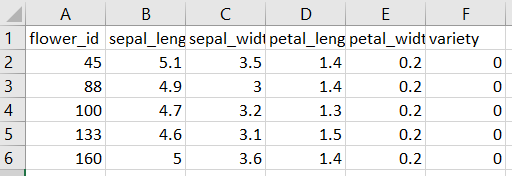
\includegraphics{figs/dataset.png}
\caption{dataset.png}
\end{figure}

    \begin{itemize}
\tightlist
\item
  Your datasets will have a \textbf{first column} with the id of each
  entry (\textbf{NOT} the same as the row index).
\end{itemize}

    \begin{itemize}
\tightlist
\item
  Your dataset will have the class/target in the \textbf{last column}.
\end{itemize}

    \begin{itemize}
\tightlist
\item
  The \textbf{first row} contains the header.
\end{itemize}

    \begin{itemize}
\tightlist
\item
  You need to find a pre-existing module that lets you import data from
  a csv file into a numpy array.
\end{itemize}

    \begin{itemize}
\tightlist
\item
  Try to import the header in a different variable as the data.
\end{itemize}

    \begin{itemize}
\tightlist
\item
  Since the classes/targets are numeric for all datasets, you can leave
  them on the same numpy array as the data.
\end{itemize}

    \begin{itemize}
\tightlist
\item
  You don't need the target names, just work with the numbers!
\end{itemize}


    % Add a bibliography block to the postdoc
    
    
    
    \end{document}
